
\tikzset{
	Commit1/.pic={
        code={
\draw[black,fill=gray, opacity=0.7] (0,0) circle (0.08cm);
\draw[black,right](-0.02,0)node[rotate=90]{\tiny \texttt{commit}};
							}
	}
}

\tikzset{
	Merge/.pic={
        code={
\draw[black,fill=gray, opacity=0.9] (0,0) circle (0.08cm);
\draw[black,left](0,0)node[rotate=90]{\tiny \texttt{merge}};
							}
	}
}

\tikzset{
	Commit2/.pic={
        code={
\draw[black,fill=gray, opacity=0.7] (0,0) circle (0.08cm);
\draw[black,left](-0.02,0)node[rotate=90]{\tiny \texttt{commit}};
							}
	}
}


\tikzset{
	Tag1/.pic={
        code={
\draw[black](-0.15,0.2)rectangle(0.15,1.2);
\draw[black](0,0.7)node[rotate=90]{\tiny \texttt{Tag V1}};
\draw[black,fill=gray, opacity=0.7] (0,0) circle (0.08cm); 
							}
	}
}

\tikzset{
	Tag2/.pic={
        code={
\draw[black](-0.15,0.2)rectangle(0.15,1.2);
\draw[black](0,0.7)node[rotate=90]{\tiny \texttt{Tag V2}};
\draw[black,fill=gray, opacity=0.7] (0,0) circle (0.08cm); 
							}
	}
}


\tikzset{
	Tag3/.pic={
        code={
\draw[black](-0.15,-1.2)rectangle(0.15,-0.2);
\draw[black](0,-0.7)node[rotate=90]{\tiny \texttt{Tag V3}};
\draw[black,fill=gray, opacity=0.7] (0,0) circle (0.08cm); 
							}
	}
}


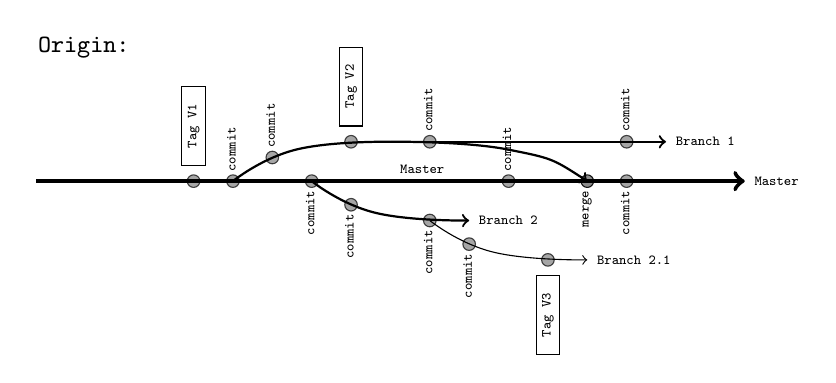
\begin{tikzpicture}
%Gitter
%\draw[step=0.5cm,very thin,black!20] (-6,-6) grid(6,6);
%\draw(-6,0)--(6,0);
%\draw(0,6)--(0,-6);

\path (-1.5,0.5) pic {Commit1};
\path (-0.5,0.5) pic {Commit2};
\path (1,1) pic {Commit1};



\path (3,0.5) pic {Merge};
\path (-2,0.5) pic {Tag1};
\path (2,0.5) pic {Commit1};
\path (3.5,1) pic {Commit1};
\path (3.5,0.5) pic {Commit2};

\path (-1,0.8) pic {Commit1};
\path (0,1) pic {Tag2};

\path (0,0.2) pic {Commit2};
\path (1,0) pic {Commit2};

\path (1.5,-0.3) pic {Commit2};
\path (2.5,-0.5) pic {Tag3};
\draw [black,ultra thick,->] plot [smooth, tension=0.8] coordinates {(-4,0.5) (5,0.5)};
\draw [black,->] plot [smooth, tension=0.8] coordinates {(1,0) (1.8,-0.4)(3,-0.5)};

\draw [black,thick] plot [smooth, tension=0.8] coordinates {(-1.5,0.5) (-0.7,0.9)(0.5,1)};

%\draw [black,thick,->] plot [smooth, tension=0.8] coordinates {(3,0.5) (3.8,0.9)(5,1)};
\draw [black,thick,->] plot [smooth, tension=0.8] coordinates {(0.5,1) (4,1)};


\draw [black,thick,<-] plot [smooth, tension=0.8] coordinates {(3,0.5) (2,0.9)(0.5,1)};


\draw [black,thick,->] plot [smooth, tension=0.8] coordinates {(-0.5,0.5) (0.3,0.1)(1.5,0)};

%\draw[black,right](0.5,1.15)node[rotate=00]{\tiny \texttt{Branch 1}};
\draw[black,right](4,1)node[rotate=00]{\tiny \texttt{Branch 1}};
\draw[black,right](0.5,0.65)node[rotate=00]{\tiny \texttt{Master}};
\draw[black,right](1.5,0)node[rotate=00]{\tiny \texttt{Branch 2}};
\draw[black,right](3,-0.5)node[rotate=00]{\tiny \texttt{Branch 2.1}};
\draw[black,right](5,0.5)node[rotate=00]{\tiny \texttt{Master}};
%\draw[black,right](4,0.5)node[rotate=00]{\small \texttt{Master}};
\draw[black,right](-4.1,2.2)node[rotate=00]{\small \texttt{Origin:}};
\end{tikzpicture}
